\chapter{Spectropolarimetry and the SALT RSS}

This chapter gives a brief overview of the basics of spectropolarimetry and how it functions based off of the principles of both spectroscopy and polarimetry. Further, it is discussed how these techniques are practically implemented for \gls{SALT}, and more specifically the \gls{RSS}, and how the spectropolarimetric reduction process is completed.

\section{Spectroscopy}

% History
Spectroscopy originated in its most basic form with Newton's examinations of sunlight through a prism \citep{opticks} but came to prominence as a field of scientific study with Wollaston's improvements to the optics elements \citep{WollPrism}, Fraunhofer's use of a diffraction grating instead of a prism as a dispersion element \citep{FraunGrating}, and Bunsen and Kirchoff's classifications of spectral features to their respective chemical elements \citep{KirBunSpec}.
\prgph

\begin{figure}[t]
    \centering
    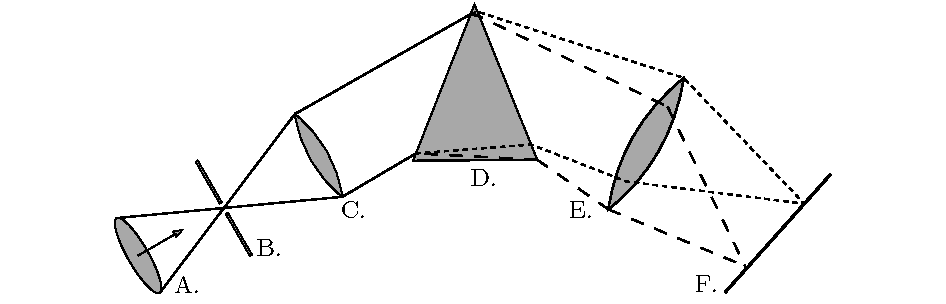
\includegraphics[width = 0.9\textwidth]{figures/2_spectrometer.pdf}
    \caption{Layout depicting the path light collected by a telescope would travel through a simple spectrometer.}
    \label{fig:spectrometer}
\end{figure}

% How it works
The simplest spectrometer schematic as shown in Figure \ref{fig:spectrometer} consists of incident light collected from the telescope's optics, labeled A, being focused onto a slit, labeled B, and passed through a collimator, labeled C. The collimator collimates the light allowing a dispersion element (such as a diffraction grating or prism), labeled D, to disperse the light into its constituent wavelengths. The resultant spectrum is focused by a focusing lens, labeled E, onto a focal plane, labeled F. Viewing optics are situated at the focal plane in the case of a spectroscope and a detector is situated at the focal plane in the case of a spectrograph.
\prgph

% Telescope optics
The telescope optics refers simply to all the components of a telescope necessary to acquire a focal point where the spectrometer, components labeled B - F, is situated. The focal point in most traditional telescope designs is fixed relative to the telescope and so the spectrometer may be mounted at that point. In cases where the telescope is designed to have a moving focal point relative to the telescope \cite[see][]{Arecibo, HET, SALT_design}, the spectrometer must also move along the telescope's focal path.
\prgph
\prgph

% SLIT
The slits function is to control the amount of incident light entering a spectrometer and, along with the exposure time of the detector, prevents over-exposures of bright sources on highly sensitive detectors \citep{TonkPracAmSpec}. If a source is spatially resolvable, or larger than the seeing conditions, the slit further acts to spatially limit the source to increase the spectral resolution, resulting in sharper features in the resultant spectrum.
\prgph

Without a slit the spectral resolution would be determined by the projected width of the source on the detector, or the seeing if the source was a star-like point source. Increasing the spectral resolution comes with the trade-off of decreasing the light collected from the source and thus acquiring a less intense resultant spectrum. Multiple spectra may be acquired simultaneously when the slit is positioned such that collinear sources lie along the slit.
%Spectroscopy done with no slit is commonly referred to as objective spectroscopy and, as the name suggests, the prism is situated just before the telescopes objective, the primary element of the telescope that focuses the collected light to the primary focus.
\prgph

% COLLIMATOR
The collimating lens functions to collimate the focused light from the telescope, ensuring that all light rays run parallel before reaching the dispersion element. Since the collimator accounts for the telescope's focus, the focal ratio of the collimator, $f_{1} / d_{1}$, should thus optimally match the focal ratio of the telescope, $f / D$, as seen in Equation \ref{eq:focal_ratio} to be most efficient and to not waste collecting area or material on too large a collimator.
% \prgph

\begin{equation}
	\frac{f}{D} = \frac{f_{1}}{d_{1}}
	\label{eq:focal_ratio}
\end{equation}

% From basic trigonometry and a small angle approximation, $\sin(\theta) \approx \theta$, Equation \ref{eq:small_angle} can be derived. From it, it can be seen that as the linear size, $D$, of most stellar objects is much smaller than the distance to those objects, $d$, and thus the incident light is already almost entirely collimated.

% \begin{equation}
% 	\theta (\arcsec) = 206265 \frac{D}{d}
% 	\label{eq:small_angle}
% \end{equation}

% DISPERSION ELEMENT
The dispersion element is the element that defines a spectrometer. As the name suggests, a dispersion element disperses the light incident on it into its constituent wavelengths and produces a spectrum. There are two types of dispersion elements, namely the prism and the diffraction grating, which operate on different principles, as discussed in Section \ref{subsec:dispersion}.
\prgph

% Focusing lens and FOCAL PLANE / Detector / Camera / CCD
% Can use \citep{CMOS_use} for CMOS use in general spectroscopy
%  - Spectroscopy and Spectrography
The focusing lens functions similarly to that of the telescope's optics but in this case focuses the dispersed light onto some receiver situated at the focal plane. As mentioned previously, an eye piece is fixed to the focal point for a spectroscope while a spectrograph employs a detector.
\prgph

The two most prevalent detector types in spectroscopy are the \gls{CCD} and \gls{CMOS} detectors. In astronomical spectroscopy however, sources are fainter and exposure times are much longer and so the \gls{CCD} detectors are by far the preferred detector as their output has a higher-quality and lower-noise when compared to \gls{CMOS} cameras under the same conditions \citep{CCDvsCMOS}.
\prgph

The \gls{CCD} is a detector composed of many thousands of pixels which can store a charge so long as a voltage is maintained across the pixels. Each pixel detects incoming photons using photo-sensitive capacitors through the photoelectric effect and converts the photons to a charge \citep{CCDastronomy}. There are also thermal agitation effects which introduce noise to the charge accumulated by a pixel, further discussed in Section \ref{subsec:calibration}. Once the exposure is finished the accumulated charge is read column by column, row by row, through an \gls{ADC}  which produces a two-dimensional array of `counts' with which information may be extracted from. Each \gls{CCD} image may be referred to by a name such as a bias, dark, flat field, or science image, which helps the observer differentiate the purpose of each image, also further discussed in Section \ref{subsec:calibration}.

\subsection{Dispersion Elements} \label{subsec:dispersion}
% https://spectroscopy.wordpress.com/2020/05/12/basics-on-prisms-and-diffraction-gratings-part-1/

Light can be broken up into its constituent wavelengths through two different physical phenomena, namely dispersion and diffraction, which dispersive elements use to create spectra. Dispersive prisms and diffractive gratings each have their strengths and weaknesses and a wide spectrum of instruments exist implementing both, or either, concepts. Regardless of the specific element, dispersive elements all have a resolving power, $R$, and an angular dispersion. Generally, while the angular dispersion is a more involved process to determine, the resolving power of a spectrograph can be measured as:
% \prgph

\begin{equation}
	R = \frac{\lambda}{FWHM}
    \label{eq:resolving_power}
\end{equation}

\noindent where $\lambda$ is the wavelength of an incident monochromatic beam and $FWHM$ refers to the width of the feature on the detector at half of its maximum intensity.
\prgph

%   - Prism
\begin{figure}[t]
    \centering
    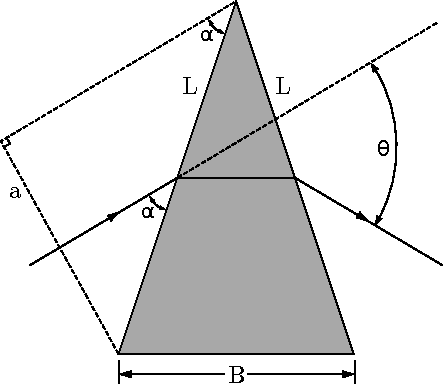
\includegraphics[width = 7cm]{figures/2_prism_diagram.pdf}
    \caption{Geometry of a prism refracting an incident monochromatic beam at a minimum deviation angle.}
    \label{fig:prism_diagram}
\end{figure}

The prism operates on the principle that the refractive index of light, $n$, varies as a function of its wavelength, $\lambda$. Prisms were the only dispersive elements available for early spectroscopic studies, but they were not without flaw.
% \prgph

\begin{equation}
	\frac{\partial \theta}{\partial \lambda} = \frac{B}{a}\frac{dn}{d\lambda}% \propto -\lambda^{-3}
    \label{eq:prism_angular_dispersion}
\end{equation}

The angular dispersion of a prism can be represented by Equation \ref{eq:prism_angular_dispersion} where the variables relate to Figure \ref{fig:prism_diagram} such that $\theta$ is the angle at which the refracted light differs from the incident light, $\lambda$ is the wavelength of the incident light, $B$ is the longest distance the beam would travel through the prism, and $a = L \sin(\alpha)$ is the cross-section of the incident beam where $L$ is the length of the transmissive surfaces and $\alpha$ is the incident angle of light to the prism surface. The refractive index of a material as a function of its wavelength, $n(\lambda)$, has several equations. Cauchy's equation, as given in Equation \ref{eq:Cauchy}, is a much simpler approximation of the refractive index that remains very accurate at visible wavelengths.
% \prgph

\begin{equation}
	n(\lambda) = A_{C} + \frac{B_{C}}{\lambda^{2}} + \frac{C_{C}}{\lambda^{4}} + \dots
    \label{eq:Cauchy}
\end{equation}

Equation \ref{eq:Cauchy}'s $A_{C}, B_{C}, C_{C}, \dots$ variables are called the Cauchy coefficients and have known values dependent on the material. Taking only the first term of the derivative of the Cauchy equation allows us to approximate the angular dispersion of a prism.

\begin{equation}
	\frac{\partial \theta}{\partial \lambda} = -\frac{B}{a}\frac{2B_{C}}{\lambda^{3}} \propto -\lambda^{-3}
    \label{eq:prism_angular_dispersion_approx}
\end{equation}

Equation \ref{eq:prism_angular_dispersion_approx} shows that the angular dispersion of a prism is wavelength dependent and furthermore that longer wavelengths are dispersed less than shorter wavelengths \citep{BirneyObsAstro, Hecht_optics}. The dependence of the angular dispersion, $d\theta/d\lambda$, on the wavelength, $\lambda$, is crucial for the formation of a spectrum but this cubic, non-linear, relation results in a non-linear spectrum. Since prisms rely on the refractive index of the material they are made of they have low angular dispersions.
\prgph

Multiple prisms can be used to increase the angular dispersion but as the dispersion is non-linear it becomes increasingly more difficult to calibrate. The more material and material boundaries the light must pass through the more its intensity decreases due to attenuation effects and Fresnel losses. Even so, the transmittance of modern prisms for their selected wavelength range is generally very high due to improved manufacturing methods as well as improved transmitting materials.
\prgph

%   - Diffraction grating
\begin{figure}[t]
    \centering
    
\includegraphics[width = 9cm]{figures/2_grating_diagram.pdf}
    \caption{Geometry of a reflective blazed grating refracting\\an incident monochromatic beam}
    \label{fig:grating_diagram}
\end{figure}

The diffraction grating operates on the principle that when light interacts with a grating where the groove size is comparable to the light's wavelength, the light is dispersed as a function of its wavelength through constructive and destructive interference. This interference results in multiple diffracted beams $m$, called orders, either side of a central reflected, or transmitted, beam such that $m \in Z$, where $m = 0$ is the non-dispersed, or reflected, beam.
% \prgph

\begin{equation}
	m\lambda = \sigma (\sin(\alpha) \pm \sin(\beta))
    \label{eq:grating_equation}
\end{equation}

% Link eq and fig
Equation \ref{eq:grating_equation} is referred to as the grating equation and its variables relate to Figure \ref{fig:grating_diagram} such that $m$ is the order of the diffracted beam being measured, $\lambda$ is the wavelength of the incident light, $\sigma$ is the groove spacing, $\alpha$ is the angle of incident light relative to the grating normal, and $\beta$ is the angle of diffraction relative to the grating normal. It is important to note that the sign of $\alpha$ and $\beta$ depend on whether the grating is reflective or transmissive. In the case of a reflective grating, such as in Figure \ref{fig:grating_diagram}, the signs of $\alpha$ and $\beta$ are the same relative to the grating normal, I.E. $\lambda = \sigma (\sin(\alpha) + \sin(\beta))$ for $m = 1$. In the case of a transmissive grating, the signs of $\alpha$ and $\beta$ are the opposite relative to the grating normal, I.E. $\lambda = \sigma (\sin(\alpha) - \sin(\beta))$ for $m = 1$.
\prgph

% Free Spectral range and Blazing
Equation \ref{eq:grating_equation} also describes how multiple wavelengths can share an angle of refraction when $m\lambda_{m} = (m + 1)\lambda_{m + 1}$. The regions of an order that do not overlap with another order are called the free spectral range. To account for the overlaps and increase the free spectral range an order-blocking filter may be used, and the diffraction grating may be blazed by an angle, $\theta$, such as in Figure \ref{fig:grating_diagram}. Blazing refers to the fact that the grooves on the surface of the grating are not symmetrical. The asymmetry of the grooves diffract the incident beam such that most of the incident beam's intensity is focused to a single order for a designated `blazed' wavelength, $\lambda_{b}$.
% \prgph

\begin{equation}
	m\lambda_{b} = 2\sigma\sin(\theta)\cos(\alpha - \theta)
    \label{eq:blaze_wavelength}
\end{equation}

\noindent where

\begin{equation}
    2\theta = \alpha + \beta
\end{equation}

% Angular dispersion
Taking the derivative of Equation \ref{eq:grating_equation} with respect to $\lambda$ and keeping $\alpha$ constant allows us to determine the angular dispersion of a diffraction grating.

\begin{equation}
    \frac{\partial \beta}{\partial \lambda} = \frac{m}{\sigma \cos(\beta)}
    \label{eq:grating_angular_dispersion}
\end{equation}

\noindent Substituting $m / \sigma$ with the grating equation gives

\begin{equation}
    \frac{\partial \beta}{\partial \lambda} = \frac{\sin(\alpha) + \sin(\beta)}{\lambda \cos(\beta)} \propto \lambda^{-1}
    \label{eq:grating_angular_dispersion_approx}
\end{equation}

Similarly to the dispersion of a prism, Equation \ref{eq:grating_angular_dispersion_approx} shows that the dispersion of a grating is wavelength dependent, but this dependence is only inversely proportional and thus more uniform across a wavelength range than that of a prism. Furthermore, shorter wavelengths are refracted less than longer wavelengths since there is no negative relation between the angular dispersion and the wavelength \citep{BirneyObsAstro, Hecht_optics}.
\prgph

% Grism and immersed grating
As mentioned before, multiple subgroups exist for both dispersive prisms and diffractive gratings. For prisms, along with the single and multiple prism setups mentioned above, there also exist grisms and immersed gratings. A grism (Grating Prism) refers to a transmissive grating etched onto one of the transmissive faces of a prism and allows a single camera to capture both spectroscopic and photometric images without needing to be moved, with and without the grism in the path of the beam of light, respectively. An immersed grating refers to a grism modified such that the transmissive grating is coated with reflective material. The primary source of dispersion for both grisms and immersive gratings is the grating and any aberration effects from the prism are negligible in comparison.
\prgph

\begin{figure}[t]
    \centering
    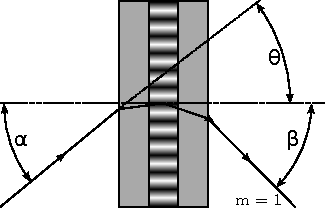
\includegraphics[width = 10cm]{figures/2_vph_grating.pdf}
    \caption{Geometry of a \gls{VPH} grating for an incident monochromatic beam of light.}
    \label{fig:vph_grating}
\end{figure}

% Echelle and VPH grating
% https://www.astro.ljmu.ac.uk/~ikb/vph.html
For gratings, along with transmissive and reflective gratings there also exist \gls{VPH} gratings. A \gls{VPH} grating consists of a photoresist, which is a light-sensitive material, sandwiched between two glass substrates. Diffraction is possible since the photoresist's refractive index varies near-sinusoidally perpendicularly to the gratings lines. This allows for sharper diffraction orders and low stray light scattering as compared to more traditional gratings but since blazing is not possible the efficiency is decreased. An echelle grating refers to two gratings set up such that the dispersed light from one is further diffracted by a second and allows for comparatively higher spectral resolutions when compared to more traditional grating setups. The gratings used as part of the echelle grating may be any type of dispersion element, but gratings are traditionally preferred due to the linearity of their resultant spectrum.
\prgph

\subsection{Detector and Spectroscopic Calibrations}\label{subsec:calibration}

Acquiring a spectrum from observations is more involved than simply reading out the data recorded on the \gls{CCD}. A raw science image, which is the raw counts of the observed source read from the \gls{CCD} with no calibrations applied, has on it a combination of useful science data as well as noise. The noise is a combination of random noise introduced through statistical processes and systematic noise introduced through the instrumentation and the observation conditions the source was observed under. This noise causes an uncertainty in the useful data and can be minimized, predominantly by calibrating for the systematic noise, but never fully removed \citep{CCDhandbook}.
\prgph

The dominant source of noise in a raw image is detector noise. \gls{CCD}'s are manufactured to have a small base charge in each pixel, called the `bias' current which allows the readout noise, a type of random noise, to better be sampled. There is also an unintentional additional charge which is linearly proportional to the exposure time and originates from thermal agitation of the \gls{CCD} material, called the `dark' current. The dark current can be minimized and possibly ignored if the \gls{CCD} is adequately cooled. These types of noise add to the charge held by a pixel and are thus considered additive.
\prgph

The \gls{CCD} is not a perfect detector and the efficiency of it and the optics of the telescope also contribute noise to the image. The efficiency of a \gls{CCD} is referred to as the Quantum Efficiency, and it is a measure of what percentage of light striking the detector is actually recorded and converted to a charge. The efficiency of the \gls{CCD} and telescope optics is also wavelength dependent and so the noise that results from them is more complex than that of additive noise. This type of noise is referred to as multiplicative noise.
\prgph

Each image taken by a \gls{CCD} will inherently have the additive types of noise in the image, and so bias and dark currents are the first types of noise to be accounted for by subtracting them from any subsequent images. Bias currents can be found by taking a bias image or by adding an overscan region to each image. A bias image is an image where the charges on the \gls{CCD} are reset and then immediately read off without exposing anything on the detector, effectively taking an image with zero exposure time. Alternatively, to save time during an observational run, overscan regions may be added to the images. An overscan region refers to adding a few cycles to the readout of each column of the \gls{CCD} such that the base current is read out and appended to each image.
\prgph

Dark currents can be found by taking an image with nothing exposed onto the detector for a certain exposure time. This resultant dark image can then be scaled to the science images exposure time since the dark current is linearly proportional to exposure time. When the detector is capable of being held at precise temperatures, dark images may be taken over multiple hours during the day to produce a high quality master dark image that may then be scaled and subtracted from all subsequent images.
\prgph

After the additive noise has been accounted for, the response from the pixels detecting the same incoming light are still not all the same due to the multiplicative noise which still needs to be accounted for. An image that has this noise accounted for is considered to be flat since all pixels share the same response to the incoming light. This noise can be measured by taking a `flat' image, or alternatively a flat-field, and multiple types of flats can be taken which all in essence image a uniformly illuminated region to determine the pixel-to-pixel response.
\prgph

Night sky flats are produced from science images where the images contain mostly sky. The science images are combined using the mode statistic which removes any celestial objects. This allows science images to be used for flat-fielding but at the cost of having a low \gls{SNR} because of the dim background sky. Dome flats are images taken of a flat surface inside the telescopes dome that has been uniformly and indirectly illuminated. These flats allow precise control of the light source and are also capable of being taken during the day. Finally, twilight flats are images taken of the twilight (or dawn) sky, when the Sun has just set, opposite the direction of the Sun at about $20\degr$ from zenith. Careful planning is required for twilight flats as the sky's brightness changes rapidly with the setting and rising of the Sun.
\prgph

A flat-field must be normalized before being used to correct any science images since it only acts to account for the pixel-to-pixel response and not for the additive errors. The normalized flat image, $F^{n}_{\lambda}(x,y)$ can be calculated as:

\begin{equation}
    F^{n}_{\lambda}(x,y) = \frac{F_{\lambda}(x,y) - B(x,y) - (\frac{t_{S}}{t_{D}})D(x,y)}{mode(F_{\lambda}(x,y) - B(x,y) - (\frac{t_{S}}{t_{D}})D(x,y))}
    \label{eq:norm_flat}
\end{equation}

\noindent where $F_{\lambda}(x,y)$ is the non-corrected flat image, $B(x,y)$ is the bias image, $D(x,y)$ is the dark image which is scaled by $t_{S}$ and $t_{D}$, the science image and dark image exposure times, respectively.
\prgph

The calibrated science image, $S^{*}_{\lambda}(x,y)$, which accounts for the bias and dark currents as well as the flat fielding can then be calculated as:

\begin{equation}
    S^{*}_{\lambda}(x,y) = \frac{S_{\lambda}(x,y) - B(x,y) - (\frac{t_{S}}{t_{D}})D(x,y)}{F^{n}_{\lambda}(x,y)}.
    \label{eq:science_cal}
\end{equation}

Multichannel \gls{CCD}'s are detectors that use either multiple \gls{CCD}'s or a \gls{CCD} with multiple output amplifiers which can be read out through multiple channels at the same time, increasing the detectors size while keeping the readout time constant. These \gls{CCD} setups need additional calibrations, specifically cross-talk corrections and mosaicking.
\prgph

Cross-talk noise refers to contamination that occurs during readout in one channel from another channel with a high signal and occurs because the signals can not be completely isolated from one another. Cross-talk corrections therefore account for this signal contamination between channels being read out at the same time \citep{CrossTalk}. Mosaicking is necessary for multichannel \gls{CCD}'s since the digitized signal read out from the detector has no reference of the physical location of the pixel it was detected at. Mosaicking therefore orients the data acquired from a multichannel detector correctly relatively to one another so that a single image is produced from the multiple channels read out from the detector.
\prgph

Finally, calibrations necessary for spectroscopy are limited to wavelength calibrations. Since the dispersion element breaks the incident light into its constituent wavelengths non-linearly, as discussed in Section \ref{subsec:dispersion}, the relation between the pixel on a detector and the wavelength of the light incident on it is unknown. Ideally, the spectrometer's optics would be modeled to produce a reliable pixel to wavelength calibration \citep[see E.g.][]{WavCalSpectraModel}, but this becomes increasingly more difficult for spectrometers with complex, non-sedentary, optical paths. Alternatively, a source with well-defined spectral features, with said features evenly populating the wavelength region of interest, such as in Figure \ref{fig:Ne_arc} may be observed. The observed frame is commonly referred to as an `arc' frame, after the arc lamps used to acquire the spectra, and should be observed alongside the science frames over the course of an observation run. It is important that the arc frame is observed at the same observing conditions and parameters as the science frames since the optical path will vary over the course of an observing run and for different observing parameters, invalidating previously acquired arc frames.
\prgph

\begin{figure}[t]
    \centering
    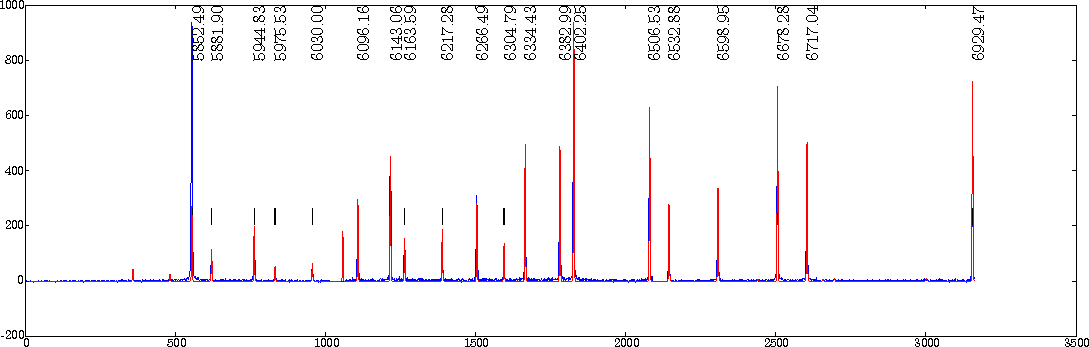
\includegraphics[width = 16cm]{figures/2_Ne_arc.pdf}
    \caption{Example of an arc spectrum for NeAr taken with \gls{SALT}'s \gls{RSS} using the PG1800 grating at a grating angle of $34.625$°, an articulation angle of $69.258$°, and covering a wavelength range of $\sim5600 - 6900$\angstrom. Plot adapted from \gls{SALT}'s published Longslit Line Atlases (as of 2023)\protect\footnotemark}
    \label{fig:Ne_arc}
\end{figure}
\footnotetext{\protect\href{http://pysalt.salt.ac.za/lineatlas/plot_line_neon.pdf}{NeAr plot} sourced from \protect\url{https://astronomers.salt.ac.za/data/salt-longslit-line-atlas/}}

The wavelength calibrations then consist of identifying a two-dimensional pixel to wavelength conversion function from the arc frame which may later be applied to calibrate the science frames. The two most common approximations for wavelength calibrations are the Chebyshev and Legendre polynomial approximations as found in Equations \ref{eq:chebyshev} and \ref{eq:legendre}, respectively. The Chebyshev polynomials are defined explicitly as:

\begin{equation}
    T_{n}(x) = \cos(n \cos^{-1}(x)),
    \label{eq:chebypolyexplicit}
\end{equation}

\noindent or recursively as:
\begin{equation}
    \begin{gathered}
        T_{0}(x) = 1 \\
        T_{1}(x) = x  \\
        T_{n}(x) = 2 x T_{n - 1}(x) - T_{n - 2}(x), \text{ for } n > 1
    \end{gathered}
    \label{eq:chebypoly}
\end{equation}

\noindent where $T$ is a Chebyshev polynomial\footnote{Denoted $T$ as a hold-over from the alternate spelling, `Tchebycheff'.} of degree $n$. Chebyshev polynomials are orthogonal when weighted by $1 / \sqrt{1 - x^{2}}$, meaning that the inner product of any two different polynomials, $T_{i}(x)$ and $T_{j}(x)$, over the range of $[-1, 1]$ is zero.

\begin{equation}
    \int_{-1}^{1} T_{i}(x) T_{j}(x) \frac{1}{\sqrt{1-x^{2}}} \,dx =
    \begin{cases}
        0,       & i \neq j\\
        \pi / 2, & i = j \neq 0\\
        \pi,     & i = j = 0
    \end{cases}
    \label{eq:chebyorth}
\end{equation}

A one or two-dimensional unknown calibration function may then be approximated by Chebyshev polynomials using:

\begin{equation}
    f(x) \approx \sum_{i = 0}^{N}  c_{i} T_{i}(u)
    \label{eq:chebyshev}
\end{equation}

\noindent or

\begin{equation}
    F(x, y) \approx \sum_{i = 0}^{N} \sum_{j = 0}^{M} c_{ij} T_{i}(u) T_{j}(v),
    \label{eq:chebyshev2D}
\end{equation}

\noindent respectively, where $N$ and $M$ are the desired $x$ and $y$ orders, $c_{ij}$ are the Chebyshev polynomial coefficients, and $u, v \in [-1, 1]$ are scaling factors to remap the variables $x, y \in [a, b]$ such that the orthogonality property of the Chebyshev polynomials holds true \citep{chebysurf, cheby2d}.

\begin{align}
    (u, v) &= \frac{2 (x, y) - a - b}{b - a} & (x, y) &= \frac{b - a}{2} (u, v) + \frac{a+b}{2}
    \label{eq:XtoUV}
\end{align}

% When the calibration function is known but the function cannot be evaluated, the coefficients, $c_{n}$, may be approximated by:

% \begin{equation}
%     c_{n} \approx \frac{2}{N} \sum_{k = 0}^{N - 1} f(x_{k}) T_{n}(x_{k})
%     \label{eq:chebycoeff}
% \end{equation}

% \noindent where:

% \noindent which returns the positions of the  x-intercepts.
% \prgph

The Chebyshev polynomials are more ideally suited for wavelength calibrations than standard polynomials since they are orthogonal and have minima and maxima located at $[-1, 1]$, as seen in Figure \ref{fig:chebyshev}. This means that the Chebyshev approximation is exact when $x = x_{n}$, where $x_{n}$ are the positions of the $n - 1$ x-intercepts of $T_{N}(x)$. This property greatly minimizes the error in the Chebyshev approximation, even at lower order approximations \citep{cheby}.

\begin{equation}
    x_{n} = \cos{\left(  \frac{\pi}{2} \frac{2 n + 1}{N} \right)}
\end{equation}

% \prgph

\begin{figure}[t]
    \centering
    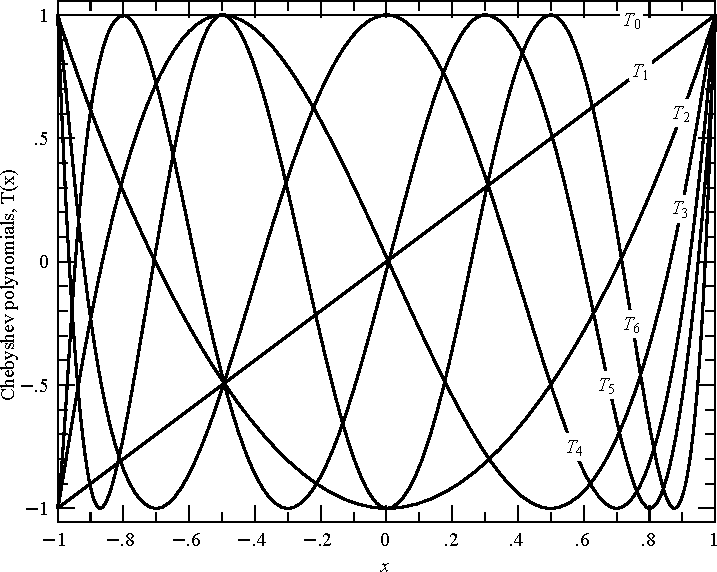
\includegraphics[width = 12cm]{figures/2_chebyshev.pdf}
    \caption{The first seven Chebyshev polynomials ($T_0$ through $T_{6}$) as defined by Equation \ref{eq:chebypoly} over the region $[-1, 1]$ for which they are orthogonal. Figure adapted from \citep{numerical_recipes} (2023)\protect\footnotemark}
    \label{fig:chebyshev}
\end{figure}
\footnotetext{Available digitally at \protect\href{http://numerical.recipes/book}{numerical.recipes}}

Similar to the Chebyshev polynomials, the Legendre polynomials may be defined explicitly as:

\begin{equation}
    P_{n}(x) = \frac{1}{2^{n} n!} \frac{d^{n}}{d x^{n}} (x^{2} - 1)^{n}
    \label{eq:legpolyexplicit}
\end{equation}

\noindent or recursively as:

\begin{equation}
    \begin{gathered}
        P_{0}(x) = 1 \\
        P_{1}(x) = x \\
        P_{n}(x) = \frac{2 n + 1}{n + 1} x P_{n - 1}(x) - \frac{n}{n + 1} P_{n - 2}(x), \text{ for } n > 1
    \end{gathered}
    \label{eq:legpoly}
\end{equation}

\noindent where P is a Legendre polynomial of degree n. Legendre polynomials are also orthogonal over the range $[-1, 1]$.
\prgph

\begin{equation}
    \int_{-1}^{1} P_{i}(x) P_{j}(x) \,dx =
    \begin{cases}
        0,                 & i \neq j\\
        \frac{2}{2 n + 1}, & i = j
    \end{cases}
    \label{eq:legorth}
\end{equation}

A one or two-dimensional unknown calibration function may then be approximated by Legendre polynomials using:

\begin{equation}
    f(x) \approx \sum_{n = 0}^{N} a_{n} P_{n}(u)
    \label{eq:legendre}
\end{equation}

\noindent or

\begin{equation}
    F(x, y) \approx \sum_{i = 0}^{N} \sum_{j = 0}^{M} a_{ij} P_{i}(u) P_{j}(v),
    \label{eq:Legendre2D}
\end{equation}

\begin{figure}[t]
    \centering
    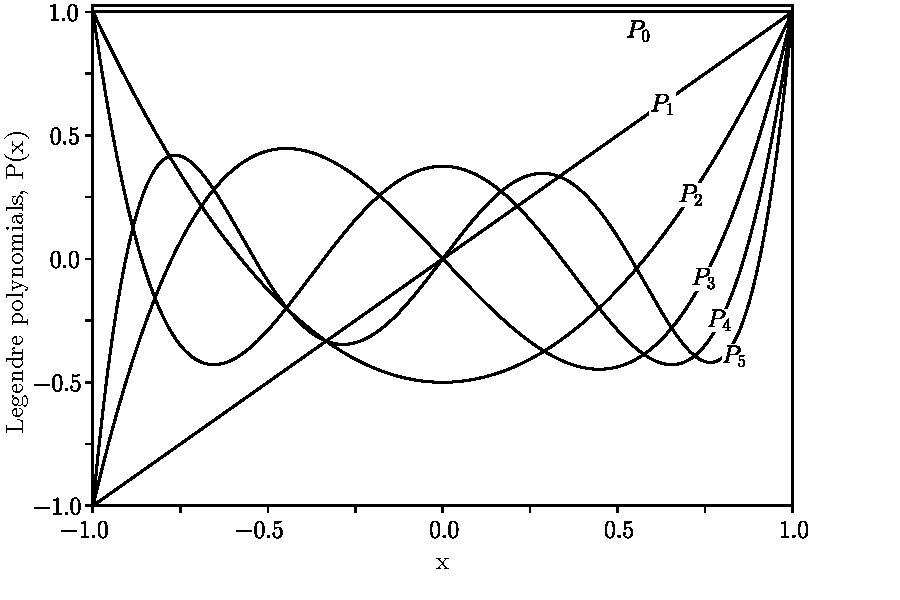
\includegraphics[width = 12cm]{figures/2_legendre.pdf}
    \caption{The first six Legendre polynomials ($P_0$ through $P_{5}$) as defined by Equation \ref{eq:legendre} over the region $[-1, 1]$ for which they are orthogonal. Figure adapted from Geek3, \protect\href{https://creativecommons.org/licenses/by-sa/3.0}{CC BY-SA 3.0}, via \protect\href{https://commons.wikimedia.org/wiki/File:Legendrepolynomials6.svg}{Wikimedia Commons} (2023)}
    \label{fig:legendre}
\end{figure}

\noindent respectively, where $N$ and $M$ are the desired $x$ and $y$ orders, $u$ and $v$ are the same mapping variable as in Equation \ref{eq:XtoUV}, and $a_{ij}$ are the Legendre polynomial coefficients. Legendre polynomials benefit from having the orthogonality condition with no weight necessary which makes their coefficients easier to compute but the error in a Legendre approximation of a function is greater than that of the error in a Chebyshev approximation for the same required order, $N$ (in one dimension) \citep{leg_cheb_relation}.
\prgph

Regardless of which set of polynomials is chosen, the polynomials are fit to the known (wavelength, pixel) pair using the least squares method. The resultant minimized function may then be used to convert the science frames from a (x pixel, y pixel) coordinate system to a (wavelength, y pixel) coordinate system.
\prgph


\section{Polarimetry}

% Origin of polarimetry (short history)
Both Huygens and Newton came to the conclusion that light demonstrates transversal properties \citep{Huygens, opticks}, which was later further investigated and coined as `polarization' by Malus \citep{Pol_Malus}. Malus also investigated the polarization effects of multiple materials including some of which were birefringent, such as optical calcite, which he referred to as Iceland spar after Bartholinus' investigations of the material \citep{Bartholinus}.

% Malus' law gives:
% \begin{equation}
%     I = I_{0} \cos^{2} \theta
%     \label{eq:Malus}
% \end{equation}
% \noindent where $I_{0}$ and $I$ are the Intensity of light before and after polarization, and $\theta$ is the orientation of the polarizer to the direction of propogation of the polarized light.
\prgph

Fresnel built on Malus' work showing that two beams of light, polarized at a right angle to one another, do not interfere, conclusively proving that light is transversal in nature, opposing the widely accepted longitudinal nature of light due to the prevalent belief in the ether. Fresnel later went on to correctly describe how polarized light is reflected and refracted at the surface of optical dielectric interfaces, without knowledge of the electromagnetic nature of light. Fresnel's equations for the reflectance and transmittance, $R$ and $T$, are defined as:

\begin{equation}
    \begin{gathered}
        R_{s} = \left\lvert \frac{Z_{2} \cos{\theta_{i}} - Z_{1} \cos{\theta_{t}}}{Z_{2} \cos{\theta_{i}} + Z_{1} \cos{\theta_{t}}} \right\rvert^{2} \\
        R_{p} = \left\lvert \frac{Z_{2} \cos{\theta_{t}} - Z_{1} \cos{\theta_{i}}}{Z_{2} \cos{\theta_{t}} + Z_{1} \cos{\theta_{i}}} \right\rvert^{2} \\
        T_{s} = 1 - R_{s} \\
        T_{p} = 1 - R_{p}
    \end{gathered}
    \label{eq:Fresnel} 
\end{equation}
    
\noindent where $s$ and $p$ are the two polarized components of light perpendicular to one another, $Z_{1}$ and $Z_{2}$ are the impedance of the two media, and $\theta_{i}$, $\theta_{t}$, and $\theta_{r}$ are the angles of incidence, transmission, and reflection, respectively \citep{Fresnel}.
\prgph

Nicol was the first to create a polarizer, aptly named the Nicol prism, where the incident light is split into its two perpendicular polarization components, namely the ordinary and extraordinary beams. Faraday discovered the phenomenon where the polarization plane of light is rotated when under the influence of a magnetic field, known as the Faraday effect. Brewster calculated the angle of incidence, $\theta_{B}$, at which incident polarized light is perfectly transmitted through a transparent surface, with refractive indexes of $n_{1}$ and $n_{2}$, while non-polarized incident light is perfectly polarized when reflected and partially polarized when refracted.

\begin{equation}
        \theta_{B} = \arctan{\frac{n_{2}}{n_{1}}}
        \label{eq:Brewster}
\end{equation}

\begin{figure}[t]
    \centering
    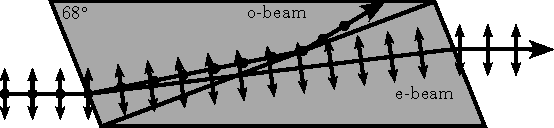
\includegraphics[width=10cm]{figures/2_Nicol_prism.pdf}
    \caption{Nicol prism diagram for incident non-polarized light.}
    \label{fig:Nicol_prism}
\end{figure}
\prgph

Stokes' work created the first consistent description of polarization and gave us the Stokes parameters which give an operational approach to polarization, discussed later in more detail \citep{Stokes}. Hale was the first to apply polarization to astronomical observations, using a Fresnel rhomb and Nicol prism as a quarter-wave plate and polarizer, respectively \citep{Hale_pre,Hale_post}. Wollaston also created a prism, similarly named the Wollaston prism, which allowed simultaneous observation of the ordinary and extraordinary beams due to the smaller deviation angle \citep{WollPrism}. Finally, Chandrasekhar's work furthered our understanding of astrophysical polarimetry by explaining the origin of polarization observed in starlight as well as mathematically modeling the polarization of rotating stars, which came to be named Chandrasekhar polarization \citep{chandrasekhar}.
\prgph

% how polarimetry works (most important) (in-depth)
% Polarimetry refers to the instrumental measurement of polarization.

% - theoretically
% Polarization ellipse from two perpendicular electric field vectors
% Maxwells electromagnetic light equations
% Stokes parameters
Maxwell's equations for an electromagnetic field propagating through a vacuum are given as:

\begin{equation}
    \begin{gathered}
        \nabla \cdot \matr{E} = 0 \\
        \nabla \cdot \matr{B} = 0 \\
        \nabla \times \matr{E} = - \frac{\partial \matr{B}}{\partial t} \\
        \nabla \times \matr{B} = \mu_{0} \epsilon_{0} \frac{\partial \matr{E}}{\partial t}
    \end{gathered}
    \label{eq:Maxwell}
\end{equation}

\noindent where $\matr{E}$ and $\matr{B}$ are the electric and magnetic field vectors, and $\mu_{0}$ and $\epsilon_{0}$ are the permeability and permittivity of free space, respectively, and related to the speed of light by $c~=~(\mu_{0} \epsilon_{0})^{-\frac{1}{2}}$. In a right-handed $(x, y, z)$ coordinate system, \hyperref[eq:Maxwell]{Maxwell's Equations} take a non-trivial solution for the electric field vector propagating along the $z$-axis, towards a hypothetical observer, of the form:

\begin{equation}
    \matr{E} = E_{x} \cos(\omega t - \Phi_{x}) \hat{\boldsymbol{x}} +
                 E_{y} \cos(\omega t - \Phi_{y}) \hat{\boldsymbol{y}}
    \label{eq:Maxwell_sol}
\end{equation}

\noindent where $E_{x}$, $E_{y}$, $\Phi_{x}$, and $\Phi_{y}$ are all constants describing the amplitude and phase of the electric field vector in the $(x, y)$ plane. Rewriting Equation \ref{eq:Maxwell_sol} using complex values allows us to simplify the form of the solution to:

\begin{equation}
    \matr{E} = \Re(\matr{E}_{0} e^{-i \omega t})
    \label{eq:E_field_vector}
\end{equation}

\noindent where we only consider the real part of the equation, and where $\matr{E}_{0}$ is defined as:

\begin{equation}
    \matr{E}_{0} = E_{x} e^{i \Phi_{x}} \hat{\boldsymbol{x}} + 
                     E_{y} e^{i \Phi_{y}} \hat{\boldsymbol{y}}
    \label{eq:pol_vector}
\end{equation}

\noindent and is referred to as the polarization vector since it neatly contains the variables that are responsible for the polarization. Although the magnetic field is not discussed, it can be shown from \hyperref[eq:Maxwell]{Maxwell's Equations} that it is always defined as in phase and perpendicular to both the electric field vector and the direction of propagation with the form $\matr{B} = \Re(\matr{B}_{0} e^{-i \omega t})$.
\prgph

% Polarizing Ellipse
For an electric field vector with oscillations in some combination of the $x$ and $y$ axes, the tip of the vector sweeps out an ellipse. This ellipse is referred to as the polarization ellipse and has the form:

\begin{equation}
    \left( \frac{\matr{E}_{x}}{\matr{E}_{0, x}}\right)^{2} +
    \left( \frac{\matr{E}_{y}}{\matr{E}_{0, y}}\right)^{2} -
    \frac{2 \matr{E}_{x} \matr{E}_{y}}{\matr{E}_{0, x} \matr{E}_{0, y}} \cos\Phi =
    \sin^{2} \Phi
    \label{eq:pol_ellipse}
\end{equation}

\noindent where $\Phi = \Phi_{x} - \Phi_{y}$ is the phase difference. The degree of polarization for the polarization ellipse is related to the eccentricity of the ellipse and the angle at which it is rotated relates to the polarization angle. Because $\matr{E}_{0, x}$, $\matr{E}_{0, y}$, $\Phi_{x}$, and $\Phi_{y}$ are constant, the resultant polarization ellipse is fixed as the wave continues to propagate. We may then manipulate Equation~\ref{eq:pol_ellipse} to produce the polarization parameters:

\begin{figure}[t]
    \centering
    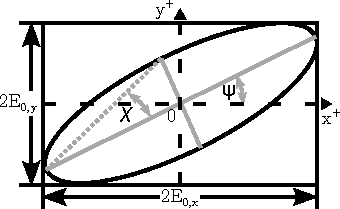
\includegraphics[width=6cm]{figures/2_pol_ellipse.pdf}
    \caption{The polarization ellipse for an electric field vector propagating through free space.}
    \label{fig:pol_ellipse}
\end{figure}


\begin{gather*}
    (E_{x}^{2} + E_{y}^{2})^{2} - (E_{x}^{2} - E_{y}^{2})^{2} - (2 E_{x} E_{y} \cos \Phi)^{2} = (2 E_{x} E_{y} \sin \Phi)^{2} \\
    \therefore P_{I}^{2} - P_{Q}^{2} - P_{U}^{2} = P_{V}^{2} \\
    \therefore P_{I}^{2} = P_{Q}^{2} + P_{U}^{2} + P_{V}^{2}
\end{gather*}

\noindent where

\begin{equation}
    \begin{gathered}
        P_{I} = E_{x}^{2} + E_{y}^{2} \\
        P_{Q} = E_{x}^{2} - E_{y}^{2} \\
        P_{U} = 2 E_{x} E_{y} \cos \Phi \\
        P_{V} = 2 E_{x} E_{y} \sin \Phi
    \end{gathered}
    \label{eq:pol_params}
\end{equation}
\prgph

There is, however, a seemingly small albeit major shortcoming of the polarization as defined in Equation~\ref{eq:pol_params}, the polarization ellipse as represented by Figure~\ref{fig:pol_ellipse} deals only with a single transverse wave and is incapable of handling a wave-packet made up of multiple waves. This is because the waves making up a wave-packet will not share their polarization properties and will temporally vary from one another. By taking the time average of the waves in a wave-packet this temporal variation may be eliminated.

\begin{equation}
    \avg{\matr{E}_{i} \matr{E}_{j}} = \lim_{T \rightarrow \infty} \frac{1}{T} \int_{0}^{T} \matr{E}_{i} \matr{E}_{j}\,dt, \text{ for } i, j \in (x, y)
\end{equation}

\noindent where $T$ is the total averaging time over electric field vectors $\matr{E}_{i}$ and $\matr{E}_{j}$. Equation~\ref{eq:pol_params} now simplifies to:

\begin{equation}
    \matr{S} = 
    \begin{pmatrix}
        S_{0} \\
        S_{1} \\
        S_{2} \\
        S_{3}
    \end{pmatrix}
    =
    \begin{pmatrix}
        I \\
        Q \\
        U \\
        V
    \end{pmatrix}
    =
    \begin{pmatrix}
        \avg{E_{x}^{2}} + \avg{E_{y}^{2}} \\
        \avg{E_{x}^{2}} - \avg{E_{y}^{2}} \\
        \avg{2 E_{x} E_{y} \cos \Phi} \\
        \avg{2 E_{x} E_{y} \sin \Phi}
    \end{pmatrix}
    \label{eq:Stokes_params}
\end{equation}

\noindent where $S_{0}$ -- $ S_{3}$ are referred to as the Stokes (polarization) parameters. This time averaging is what previous definitions of polarization failed to account for and as such they were only able to account for beams of completely polarized light. For a reference direction which defines the direction of the $x$-axis of our coordinate system, the Stokes parameters are physically described as follows: the $Q$ Stokes parameter is defined as the difference between the amount of photons oscillating parallel and perpendicular to the reference direction, the $U$ Stokes parameter is defined as the difference between the amount of photons oscillating at $45\degr$ and $135\degr$ counter-clockwise from the reference direction, and the $V$ Stokes parameter is defined as the difference between the amount of photons with right-handed (positive, clockwise) circular polarization and left-handed (negative, counter-clockwise) circular polarization \citep{Stokes}.
\prgph

Using the \hyperref[eq:Stokes_params]{Stokes parameters}, we can now account for partially polarized light such that:

\begin{equation}
    I^{2} \geq  Q^{2} + U^{2} + V^{2},
\end{equation}

\noindent where it should be noted that $(I, Q, U, V)$ represent the partial polarization parameters and are related to $(P_{I}, P_{Q}, P_{U}, P_{V})$ since the polarization may be partial. In general, and henceforth, $(P_{I}, P_{Q}, P_{U}, P_{V})$ are relative quantities normalized to the intensity, where

\begin{align}
    P_{I} &= 1, & P_{Q} &= \frac{Q}{I}, & P_{U} &= \frac{U}{I}, \text{   and } & P_{V} &= \frac{V}{I}.
    \label{eq:norm_Stokes}
\end{align}
\prgph

Similar to the polarization ellipse, the Stokes parameters may be represented pictorially using the Poincar{\'e} sphere in spherical coordinates $(IP, 2 \Psi, 2 \chi)$, where $I$ denotes the total intensity and $P$ the degree of polarization, or the ratio of polarized to non-polarized light in the wave-packet, $\Psi$ denotes the polarization angle. It should be noted that the Poincar{\'e} sphere also uses the normalized Stokes parameters $(S_{0} = 1)$ as defined above in equation~\ref{eq:norm_Stokes}.

\begin{equation}
    \begin{gathered}
        I = S_{0} \\
        P = \frac{\sqrt{S_{1}^2 + S_{2}^2 + S_{3}^2}}{S_{0}}, \text{ for } 0 \leq P \leq 1 \\
        2 \Psi = \arctan \frac{S_{2}}{S_{1}} \\
        2 \chi = \arctan \frac{S_{3}}{\sqrt{S_{1}^{2} + S_{2}^{2}}}
    \end{gathered}
    \label{eq:poincare_coords}
\end{equation}

\begin{figure}[t]
    \centering
    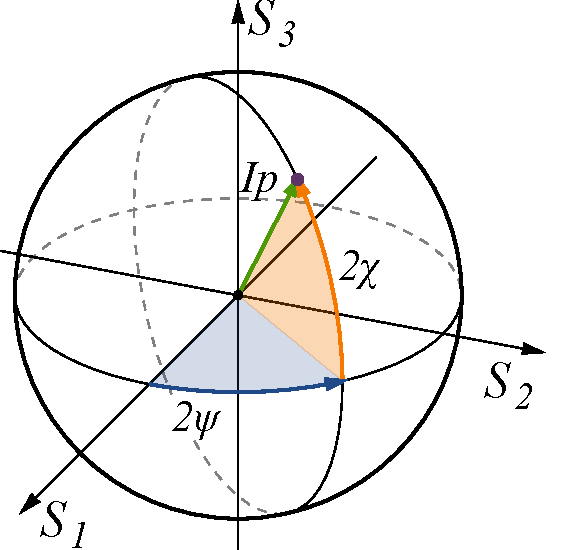
\includegraphics[width=6cm]{figures/2_poincare_sphere.pdf}
    \caption{The Poincar{\'e} sphere describing the polarization properties of a wave-packet propagating through free space. Figure adapted from Inductiveload, via \protect\href{https://commons.wikimedia.org/wiki/File:Poincaré_sphere.svg}{Wikimedia Commons} (2023)}
    \label{fig:poincare}
\end{figure}
\prgph

% The now time-invariant \hyperref[fig:pol_ellipse]{polarization ellipse} may now be defined in terms of the Stokes parameters as:

% Special cases, (1, \pm1, 0, 0), (1, 0, \pm1), (1, 0, 0, \pm1), (1, 0, 0, 0)
% Mueller matrix
% \citep{pol_in_spectra}

\begin{figure}[t]
    \centering
    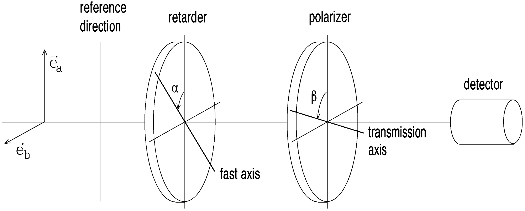
\includegraphics[width=1\textwidth]{figures/2_polarimeter.pdf}
    \caption{Diagram of an ideal polarimeter. Figure adapted from \cite{pol_in_spectra}.}
    \label{fig:polarimeter}
\end{figure}

% - practically
% Waveplate and polarizer
Except for polarimetry in the radio-wavelength regime, the polarization of a beam can not be directly measured. The polarization properties may, however, be recovered from the beam through manipulation of the four constants mentioned in Equation~\ref{eq:Maxwell_sol}. This so-called manipulation is achieved by passing the beam through optical elements which vary the beam for differing amplitudes and phases. These matrix operations may be represented by their corresponding Mueller matrices. For ideal components, the resultant beam $\matr{S}^{\prime}$ after passing through an optical element is given by

\begin{equation}
    \matr{S}^{\prime} = \matr{M} \matr{S}
\end{equation}

\noindent where $\matr{S}$ is the beam incident on the optical element and $\matr{M}$ represents the $4 \times 4$ Mueller matrix representing the optical element. Mueller matrices are especially useful when dealing with paths through optical elements as they observe the `train' property \citep{Mueller_train}. This means that an incoming beam $\matr{S}$ passing, in order, through elements with known Mueller matrices $(\matr{M}_{0}, \dots, \matr{M}_{N})$ results in an outgoing beam $\matr{S}^{\prime}$ such that:

\begin{equation}
    \matr{S}^{\prime} = \matr{M}_{N} \dots \matr{M}_{0} \matr{S}
    \label{eq:mueller_train}
\end{equation}

Some Mueller Matrices are given below with angles related to those in Figure~\ref{fig:polarimeter}, measured counter-clockwise in a right-handed coordinate system.

\paragraph*{General rotation}
The Mueller matrix for coordinate space rotations about the origin by an angle $\theta$.
\begin{equation}
    \matr{R}(\theta) = 
    \begin{bmatrix}
        1 &  0             & 0             & 0 \\
        0 &  \cos 2 \theta & \sin 2 \theta & 0 \\
        0 & -\sin 2 \theta & \cos 2 \theta & 0 \\
        0 &  0             & 0             & 1 \\
    \end{bmatrix}
    \label{matrix:rotate}
\end{equation}

\paragraph*{General linear retardance}
The Mueller matrix for retardance where $\alpha$ is the angle between the incoming vector and fast axis, and $\delta$ is the retardance introduced by the retarder. The retarder is often referred to by this retardance, e.g. if the retardance is $\delta = \pi$ or $\pi / 2$ $radians$, the retarder is referred to as a half- or quarter-wave plate, respectively.
\begin{equation}
    \matr{W}(\alpha, \delta) = 
    \begin{bmatrix}
        1 & 0               & 0               & 0 \\
        0 & \cos^{2} 2 \alpha + \sin^{2} 2 \alpha \cos \delta & \cos 2 \alpha \sin 2 \alpha  (1 - \cos \delta) & \sin 2 \alpha \sin \delta \\
        0 & \cos 2 \alpha \sin 2 \alpha  (1 - \cos \delta) & \cos^{2} 2 \alpha \cos \delta + \sin^{2} 2 \alpha & -\cos 2 \alpha \sin \delta \\
        0 & -\sin 2 \alpha \sin \delta& \cos 2 \alpha \sin \delta & \cos \delta \\
    \end{bmatrix}
    \label{matrix:retarder}
\end{equation}

\paragraph*{General linear polarization}
The Mueller matrix for linear polarization where $\beta$ is the angle between the incoming vector and transmission axis.
\begin{equation}
    \matr{P}(\beta) = \frac{1}{2}
    \begin{bmatrix}
        1            & \cos 2 \beta              & \sin 2 \beta              & 0 \\
        \cos 2 \beta & \cos^{2} 2 \beta          & \cos 2 \beta \sin 2 \beta & 0 \\
        \sin 2 \beta & \sin 2 \beta \cos 2 \beta & \sin^{2} 2 \beta          & 0 \\
        0            & 0                         & 0                         & 0 \\
    \end{bmatrix}
    \label{matrix:polarizer}
\end{equation}
\prgph


These matrices in combination with the chain rule in Equation~\ref{eq:mueller_train} allow us to describe how the Stokes parameters would change when passing through various optical elements. For a setup similar to Figure~\ref{fig:polarimeter}, we can vary the polarization angle, $\alpha$, and retandance angle, $\beta$, to acquire a system of equations that we can solve to retrieve the Stokes polarization parameters.

\begin{equation}
    I(\alpha, \beta) = \frac{1}{2} \left[ I + Q \cos2\beta + U \cos\alpha \sin2\beta + V \sin\alpha \sin2\beta\right]
\end{equation}

% Wollaston prism, hwp, etc.





\subsection{Polarimetric calibrations}

% Wollaston corrections
% Tilt corrections


\section{Spectropolarimetry} % In depth

% Spectropolarimetry is composed of Spectroscopy and polarimetry ...

% Origin of spectropolarimetry (short history)
% how spectropolarimetry works in-depth (both practically and theoretically, I.E. frames, traces, O and E beams, etc).

% Uses and what its use in astrophysics is.




\section{The South African Large Telescope} % Basics, not in depth

\gls{SALT} is a 10 m class optical/near-infrared telescope situated at the \gls{SAAO} field station near Sutherland, South Africa \citep{SALT_optical_design}. The operational design was based off of the \gls{HET} situated at McDonald Observatory, Texas, which limits the pointing of the telescope's primary mirror to a fixed elevation (37$\degree$ from zenith in the case of SALT) while still allowing for full azimuthal rotation \citep{HET}. Both SALT and HET utilize a spherical primary mirror which is stationary during observations and a tracker housing most of the instrumentation that tracks the primary mirrors spherically shaped focal path. Figure \ref{fig:SALT_telescope} depicts \gls{SALT}'s tracker (top left), supporting structure, and primary mirror (bottom right).

\begin{figure}[t]
    \centering
    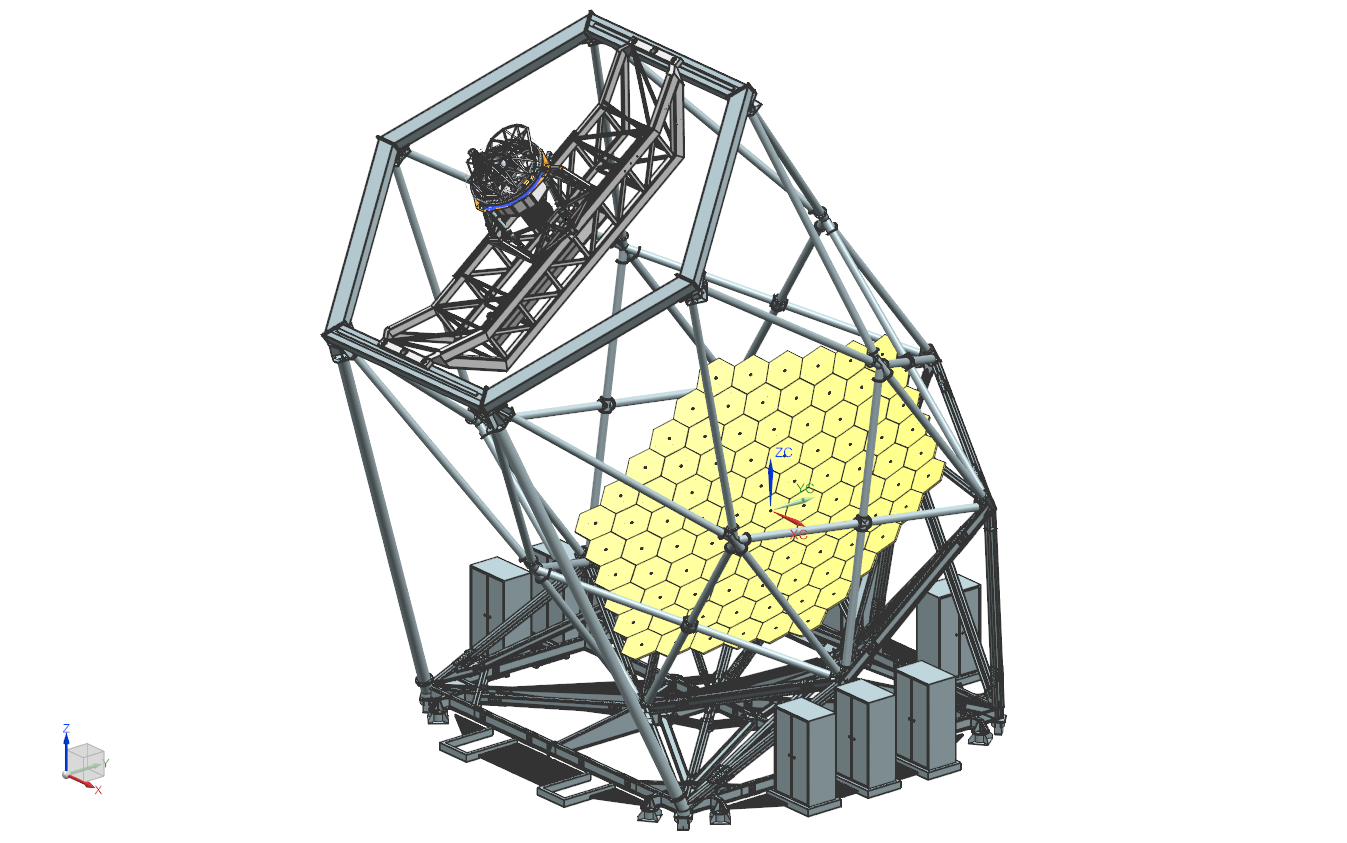
\includegraphics[width = 15cm]{figures/2_SALT_telescope.png}
    \caption{The tracker, supporting structure, and primary mirror of SALT. Figure adapted from the SALT call for proposals (2022)\protect\footnotemark}
    \label{fig:SALT_telescope}
\end{figure}
\footnotetext{\protect\url{http://pysalt.salt.ac.za/proposal_calls/current/ProposalCall.html}}

\subsection{The primary mirror}

The primary mirror is composed of 91 individual 1 m hexagonal mirrors which together form an 11 m segmented spherical mirror. Each mirror segment can be adjusted by actuators allowing the individual mirrors to approximate a single monolithic spherical mirror. The fixed elevation means that SALT's primary mirror has a fixed gravity vector allowing for a lighter, cost-effective supporting structure when compared to that of a more traditional altitude-azimuthal mount but with the trade-off that the control mechanism and tracking has increased complexity \citep{SALT_design}.

\subsection{Tracker and tracking}

During observations the primary mirror is stationary and the tracker tracks celestial objects across the sky by moving along the primary focus. The tracker is capable of 6 degrees of freedom with an accuracy of ~5 $\mu$m and is capable of tracking $\pm$6$\degree$ from the optimal central track position. Targets at declinations from 10.5$\degree$ to -75.3$\degree$, as shown in Figure \ref{fig:SALT_visibility} are accessible during windows of opportunity. As the tracker moves along the track the effective collecting area varies and thus SALT has a varying effective diameter of $\sim7$ m to 9 m when the tracker is furthest and closest to the optimal central position, respectively.
\prgph

\begin{figure}[t]
    \centering
    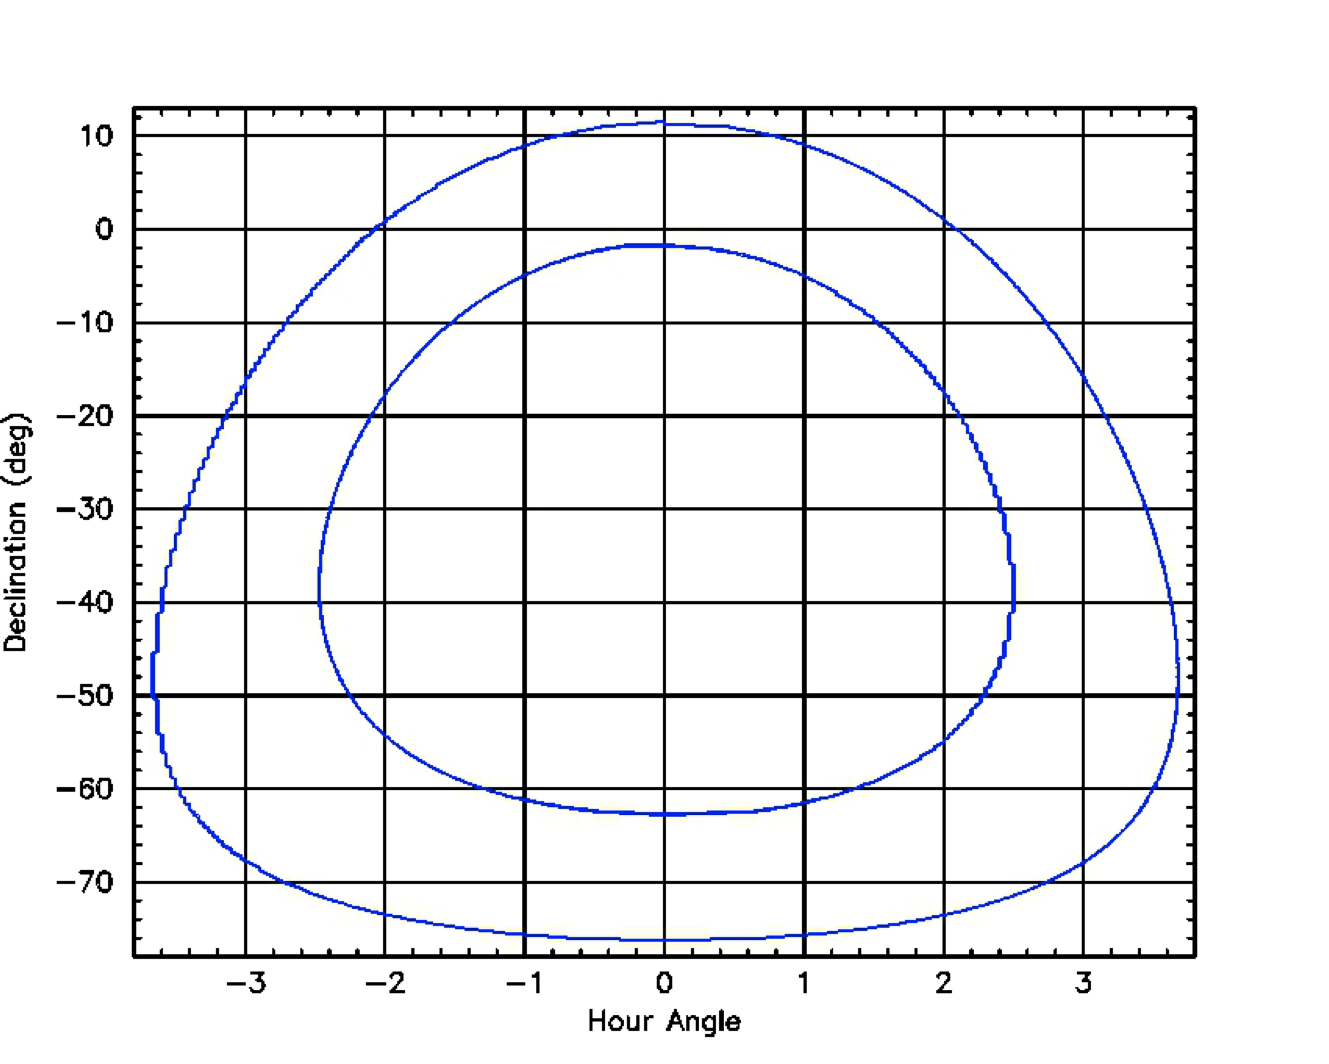
\includegraphics[width = 13cm]{figures/2_SALT_visibility.png}
    \caption{The visibility annulus of objects observable by SALT. Figure adapted from the SALT call for proposals (2013)\protect\footnotemark}
    \label{fig:SALT_visibility}
\end{figure}
\footnotetext{\protect\url{https://pysalt.salt.ac.za/proposal_calls/2013-2/}}

% Mention Center of Curvature Alignment System? : https://en.wikipedia.org/wiki/Shack%E2%80%93Hartmann_wavefront_sensor

The tracker is equipped with a 4 mirror spherical aberration corrector \citep{SALT_SAC}, and an atmospheric dispersion compensator \citep{SALT_ADC}, which corrects for the spherical aberration caused by the geometry of the primary mirror and allows access to wavelengths as short as 3200 \AA. These return a corrected flat focal plane with an 8\arcmin diameter field of view at prime focus on to the science instruments, with a 1\arcmin annulus around it used by the Tracker in a closed-loop guidance system.
\prgph

\subsection{The Robert Stobie Spectrograph}

SALT is equipped with the \gls{SALTICAM} and the \gls{RSS} science instruments onboard the tracker, and the \gls{HRS} and \gls{NIRifs} science instruments which are fibre-fed from the tracker to their own climate controlled rooms. The \gls{RSS} is the most used instrument on \gls{SALT} and the only instrument used for spectropolarimetry, and as such will be discussed in more depth than the other instruments.

The \gls{NIRifs} is currently being commissioned and will extend SALT's operational wavelength range from 3200 - 9000 \AA\ to 3200 - 17000 \AA, providing medium resolution spectroscopy at R = 2000 - 5000 over NIR wavelengths \citep{NIR, SALT_NIR}. This is ideally suited for studies of nearby galaxies.

The \gls{HRS} echelle spectrograph was designed for high resolution spectroscopy at R = 37000 - 67000 covering a wavelength range of 3700 - 8900 \AA\ and consists of a dichroic beam splitter and two \gls{VPH} gratings \citep{SALT_hires}. This instrument is capable of stellar atmospheric and radial velocity analysis.

The SALTICAM functions as the acquisition camera and simple science imager with various imaging modes, such as full-mode and slot-mode imaging, and supports low exposure times, down to 50 ms \citep{SALTICAM}. This enables photometry of faint objects, especially at fast exposure times.
\prgph

The \gls{RSS} functions as the primary spectrograph on \gls{SALT} and can operate in long-slit spectroscopy and spectropolarimetry modes, narrowband imaging mode, multi-object and high resolution spectroscopy modes, and low resolution Fabry-P\'erot imaging spectroscopy and tunable filter narrowband imaging modes \citep[for an in-depth discussion on operational modes see][]{SALT_operational_modes}.
\prgph

TODO: Optical layout (Figure) and description, and CCD/Lamps/Filters etc. available. Focus on spectropolarimetry and a short description on how observations are organized, gratings, spectral ranges, as well as the latest developments (PG0700, and anything else new)
\prgph

\section{RSS Spectropolarimetric Reductions} % In depth

TODO: How spectropolarimetry reductions differ from spectroscopy, polarimetry, and general spectropolarimetry reductions

\subsection{General Reduction Process} % Rename?, In depth

TODO: How reductions would be done in general and through pure IRAF.

I.E. Frames observed → flat, bias, arc, multiple targets, others(?)

Corrections → flat fielding, bias subtraction (EQ from obs. astro), others(?)

Calibrations → wavelength, flux, shifting (trace to center), background subtraction, others(?)

Extraction → spectral extraction, others(?)

\sout{Stokes parameter calculations / Post processing / Displaying / saving / comparing results}

\subsection{POLSALT} % In depth

TODO:

In depth but not a users guide, more focus on purpose than the parameters (I.E. why each step is necessary and draw comparison to general reduction)

Why polsalt works without any major need for concern. "All steps except for the wavelength calibration and spectral extraction run with no user input. The spectral extraction is not a calibration but a simple check to make sure the entire trace is included in the window and also that the background regions do not contain any other objects lying on the frame or include the trace."

\noindent Raw image reductions

[Bias/Dark/Flat/Fringe(?)/Crosstalk/Mosaicking]
All processes run / files created / PURPOSE!

\noindent Wavelength calibrations

[Arc/Background subtraction/Cosmic ray rejection]
All processes run / files created / PURPOSE! / Heavy focus since supplementary pipeline replaces this step

\noindent Spectral extraction

All processes run / files created / PURPOSE!

\noindent Raw Stokes calculations

[Wollaston]
All processes run / files created / PURPOSE!

\noindent Final Stokes calculations

All processes run / files created / PURPOSE!

\noindent Post-processing analysis % All 'script.py' steps in the BASH reduction

PURPOSE
Data Culling (BASH) (not used but mention use) / 
Flux Calibrations (BASH and errors in GUI (make 100\% sure about division error and notify Danielle before/if planning on including)) / 
saving plot and text pipeline results (BASH and GUI) / 
Synthetic Filtering (BASH) / 

Mention bash script and GUI versions and differences, as well as what SALT's preferred method is
